%\documentclass[11pt,handout]{beamer}
\documentclass[9pt]{beamer}
\usetheme[white]{Illinois}

\title[]{Micro-reactor evaluation for hydrogen economy}
% \subtitle[]{}
\author[]{\textbf{Roberto Fairhurst Agosta}}
\date[12.02.2020]{December 2, 2020}
\institute[UIUC]{Advanced Reactors and Fuel Cycles\\University of Illinois at Urbana-Champaign}

%\usepackage{bbding}
\usepackage{amsfonts}
\usepackage{amsmath}
\usepackage{xspace}
\usepackage{graphicx}
\usepackage{subfigure}
\usepackage{booktabs} % nice rules for tables
\usepackage{microtype} % if using PDF
\usepackage{bigints}
\usepackage{minted}
\usepackage[absolute,overlay]{textpos}
\usepackage{tikz}
\usetikzlibrary{positioning, arrows, decorations, shapes}
\usetikzlibrary{shapes.geometric,arrows}
\definecolor{illiniblue}{HTML}{B1C6E2}
\tikzstyle{bblock} = [rectangle, draw, fill=illiniblue,
text width=10em, text centered, rounded corners, minimum height=4em]
\tikzstyle{sbblock} = [rectangle, draw, fill=illiniblue,
text width=7em, text centered, rounded corners, minimum height=4em]
\tikzstyle{arrow} = [thick,->,>=stealth]

\newcommand{\units}[1] {\:\text{#1}}%
\newcommand{\SN}{S$_N$}%{S$_\text{N}$}%{$S_N$}%
\DeclareMathOperator{\erf}{erf}
\DeclareMathOperator{\erfc}{erfc}
\setbeamertemplate{bibliography item}[text]

%%%% Acronym support
\usepackage[acronym,toc]{glossaries}
\newacronym{ANL}{ANL}{Argonne National Laboratory}
\newacronym{API}{API}{Application Programming Interface}
\newacronym{B4C}{B4C}{boron carbide}
\newacronym{BC}{BC}{boundary condition}
\newacronym{BOC}{BOC}{beginning of the equilibrium cycle}
\newacronym{BSD}{BSD}{Berkeley Software Distribution}
\newacronym{BWR}{BWR}{Boiling Water Reactor}
\newacronym{CAISO}{CAISO}{California ISO}
\newacronym{CAPP}{CAPP}{Core Analyzer for Pebble and Prism type VHTRs}
\newacronym{CEA}{CEA}{Commissariat a l'Energie Atomique}
\newacronym{CFD}{CFD}{computational fluid dynamics}
\newacronym{CO2}{CO$_2$}{carbon dioxide}
\newacronym{CR}{CR}{control rod}
\newacronym{CRP}{CRP}{Coordinated Research Project}
\newacronym{CZP}{CZP}{Cold Zero Power}
\newacronym{DCC}{DCC}{depressurized conduction cool-down}
\newacronym{DOE}{DOE}{Department of Energy}
\newacronym[\glslongpluralkey={degrees of freedom}]{DoF}{DoF}{degree of freedom}
\newacronym{EOC}{EOEC}{end of the equilibrium cycle}
\newacronym{FCEV}{FCEV}{Fuel Cell Electric Vehicle}
\newacronym{FDM}{FDM}{Finite Difference Method}
\newacronym{FEM}{FEM}{Finite Element Method}
\newacronym{FVM}{FVM}{Finite Volume Method}
\newacronym[\glslongpluralkey={greenhouse gases}]{GHG}{GHG}{greenhouse gas}
\newacronym{GRS}{GRS}{Gesellschaft für Anlagen und Reaktorsicherheit}
\newacronym{GT-MHR}{GT-MHR}{Gas Turbine-Modular Helium Reactor}
\newacronym{H2}{H$_2$}{hydrogen}
\newacronym{He}{He}{helium}
\newacronym{HFP}{HFP}{Hot Full Power}
\newacronym{HPCC}{HPCC}{high-pressure conduction cool-down}
\newacronym{HTE}{HTE}{High-Temperature Electrolysis}
\newacronym{HTGR}{HTGR}{High-Temperature Gas-Cooled Reactor}
\newacronym{HTR}{HTR}{High Temperature Reactor}
\newacronym{HTTR}{HTTR}{High-Temperature engineering Test Reactor}
\newacronym{HZDR}{HZDR}{Helmholtz-Zentrum Dresden-Rossendorf}
\newacronym{IAEA}{IAEA}{International Atomic Energy Agency}
\newacronym{icap}{iCAP}{Illinois Climate Action Plan}
\newacronym{INL}{INL}{Idaho National Laboratory}
\newacronym{IPyC}{IPyC}{inner pyrolytic carbon}
\newacronym{JFNK}{JFNK}{Jacobian-Free Newton-Krylov}
\newacronym{KAERI}{KAERI}{Korea Atomic Energy Research Institute}
\newacronym{Keff}{k$_{eff}$}{multiplication factor}
\newacronym{LBP}{LBP}{Lumped Burnable Poison}
\newacronym{LGPL}{LGPL}{Lesser GNU Public License}
\newacronym{LOCA}{LOCA}{loss of coolant accident}
\newacronym{LPCC}{LPCC}{low-pressure conduction cool-down}
\newacronym{LTE}{LTE}{Low-Temperature Electrolysis}
\newacronym{LWR}{LWR}{Light Water Reactor}
\newacronym{MC}{MC}{Monte Carlo}
\newacronym{MHTGR}{MHTGR}{Modular High-Temperature Gas-Cooled Reactor}
\newacronym{MMR}{MMR}{Micro Modular Reactor}
\newacronym{MOC}{MOC}{middle of the equilibrium cycle}
\newacronym{MOX}{MOX}{mixed-oxide}
\newacronym{MOOSE}{MOOSE}{Multi-physics Object-Oriented Simulation Environment}
\newacronym{MPI}{MPI}{Message Passing Interface}
\newacronym{MSR}{MSR}{Molten Salt Reactor}
\newacronym{MTD}{MTD}{Champaign-Urbana Mass Transit District}
\newacronym{NEA}{NEA}{Nuclear Energy Agency}
\newacronym{NEM}{NEM}{Nodal Expansion Method}
\newacronym{NGNP}{NGNP}{Next Generation Nuclear Power}
\newacronym{NRC}{NRC}{Nuclear Regulatory Commission}
\newacronym{NSC}{NSC}{Nuclear Science Committee}
\newacronym{OECD}{OECD}{Organisation for Economic Co-operation and Development}
\newacronym{OPyC}{OPyC}{outer pyrolytic carbon}
\newacronym{ORNL}{ORNL}{Oak Ridge National Laboratory}
\newacronym{OS}{OS}{Operator-Splitting}
\newacronym{PBMR}{PBMR}{Pebble Bed Modular Reactor}
\newacronym{PDE}{PDE}{Partial Differential Equation}
\newacronym{PMR}{PMR}{Prismatic Modular Reactor}
\newacronym{PV}{PV}{photovoltaics}
\newacronym{RPV}{RPV}{Reactor Pressure Vessel}
\newacronym{RSC}{RSC}{Reserve Shutdown Control}
\newacronym{RSD}{RSD}{Relative Standard Deviation}
\newacronym{SD}{SD}{Standard Deviation}
\newacronym{SI}{SI}{Sulfur-Iodine}
\newacronym{SiC}{SiC}{silicon carbide}
\newacronym{SMR}{SMR}{Small Modular Reactor}
\newacronym{SNU}{SNU}{Seoul National University}
\newacronym{SOEC}{SOEC}{Solid Oxide Electrolysis Cells}
\newacronym{SP3}{SP$_3$}{Simplified P$_3$}
\newacronym{TIP}{TIP}{transverse integration procedure}
\newacronym{TRISO}{TRISO}{Tristructural Isotropic}
\newacronym{UIUC}{UIUC}{University of Illinois at Urbana-Champaign}
\newacronym{UNIST}{UNIST}{Ulsan National Institute of Science and Technology}
\newacronym{UK}{UK}{United Kingdom}
\newacronym{UMICH}{UMICH}{University of Michigan}
\newacronym{US}{US}{United States}
\newacronym{USNC}{USNC}{Ultra Safe Nuclear Corporation}
\newacronym{VHTR}{VHTR}{Very High-Temperature Gas-Cooled Reactor}
%\newacronym{<++>}{<++>}{<++>}
%\newacronym{<++>}{<++>}{<++>}

\makeglossaries

%try to get rid of header on title page\dots
\makeatletter
\newenvironment{withoutheadline}{
  \setbeamertemplate{headline}[default]
  \def\beamer@entrycode{\vspace*{-\headheight}}
}{}

\makeatother
\makeatother
\setbeamertemplate{footline}
{
  \leavevmode%
  \hbox{%
    \rightline{\insertframenumber{} / \inserttotalframenumber\hspace*{1ex}}
  }%
  \vskip0pt%
}
\makeatletter

\begin{document}
\newcommand*{\alphabet}{ABCDEFGHIJKLMNOPQRSTUVWXYZabcdefghijklmnopqrstuvwxyz}
\newlength{\highlightheight}
\newlength{\highlightdepth}
\newlength{\highlightmargin}
\setlength{\highlightmargin}{2pt}
\settoheight{\highlightheight}{\alphabet}
\settodepth{\highlightdepth}{\alphabet}
\addtolength{\highlightheight}{\highlightmargin}
\addtolength{\highlightdepth}{\highlightmargin}
\addtolength{\highlightheight}{\highlightdepth}
\newcommand*{\Highlight}{\rlap{\textcolor{HighlightBackground}{\rule[-\highlightdepth]{\linewidth}{\highlightheight}}}}

\begin{withoutheadline}
\frame{
  \titlepage
}
\end{withoutheadline}

%%--------------------------------%%
\AtBeginSection[]{
\begin{frame}
  \frametitle{Outline}
  \tableofcontents[currentsection]
\end{frame}
}

\section{Introduction}
\subsection{Objectives}
\begin{frame}
\frametitle{Objectives}
  \begin{itemize}
    \item Implement and solve $SP_3$ equations with a MOOSE-based application for the following cases:
    \item one-dimensonal models:
	\begin{itemize}
		\item fixed source problem with one energy group,
		\item eigenvalue problem with one energy group,
		\item fixed source problem with multiple energy groups,
		\item eigenvalue source problem with multiple energy groups,
		\item compare results to diffusion solver,
	\end{itemize}
    \item two-dimensonal model: C5 MOX Benchmark \cite{capilla_applications_2009}.
  \end{itemize}
\end{frame}


\section{Hydrogen Production Methods}
\subsection{Electrolysis}
\begin{frame}
\frametitle{Electrolysis}
\begin{columns}
    \column[t]{5cm}
	\begin{figure}[htbp!]
		\begin{center}
			\includegraphics[height=3.6cm]{images/hte-energy-P.png}
		\end{center}
		\caption{Energy required by HTE at 3.5 MPa.}
	\end{figure}

	\column[t]{5cm}
	$\Delta H = \Delta G + T \Delta S$
	\begin{itemize}
		\item $\Delta$G: specific electrical energy $kWh \cdot kg_{H_2}^{-1}$
		\item T$\Delta$S: specific thermal energy $kWh \cdot kg_{H_2}^{-1}$.
	\end{itemize}
    \vspace{0.7cm}

	\begin{itemize}
    	\item In low temperature electrolysis (LTE), electricity provides the thermal energy.
    	\item In high temperature electrolysis (HTE), a heat source provides the thermal energy.
    	\item HTE has the advantage of decreasing the electricity requirement.
    \end{itemize}
\end{columns}
\end{frame}

\subsection{Sulfur-Iodine}
\begin{frame}
\frametitle{Sulfur-Iodine}
\begin{columns}
    \column[t]{5cm}
  	\begin{figure}[htbp!]
		\begin{center}
			\includegraphics[width=5cm]{images/sulfur1.png}
		\end{center}
		\caption{Diagram of the Sulfur-Iodine Thermochemical process.}
 	\end{figure}

 	\column[t]{5cm}
   	\begin{figure}[htbp!]
		\begin{center}
			\includegraphics[width=4.8cm]{images/si-energy2.png}
		\end{center}
		\caption{Energy required by the Sulfur-Iodine Thermochemical Cycle.}
 	\end{figure}
\end{columns}
\end{frame}

\begin{frame}
\frametitle{Co-generation}
\begin{columns}
    \column[t]{5cm}
  	\begin{figure}[htbp!]
		\begin{center}
			\includegraphics[width=4.5cm]{images/hte-figure0.png}
		\end{center}
		\caption{Diagram of a reactor coupled to a hydrogen plant.}
 	\end{figure}

 	\column[t]{5cm}
	\begin{table}[!htb]
		\centering
	    \caption{Energy requirements of the different H$_2$ production methods.}
		\begin{tabular}{cccc}
	\hline
    Method    & $\gamma$         & $P_{EH2}$ & $P_{TH2}$ \\ \hline
    LTE & 1                & $\ne$ 0   & 0         \\ 
    HTE & $0 < \gamma < 1$ & $\ne$ 0   & $\ne$ 0   \\ 
    SI  & 0                & 0         & $\ne$ 0   \\ \hline
        \end{tabular}
	\end{table}
\end{columns}
\end{frame}

	% \begin{table}[!htb]
	% 	\centering
	%     \caption{GGE, DGE, and E85GE \cite{doe_office_of_energy_efficiency_and_renewable_energy_hydrogen_2020} \cite{alternative_fuels_data_center_fuel_2014}.}
	% 	\begin{tabular}{l|l}
	% 	\hline
	% 	                 & Hydrogen \\ \hline
	% 	GGE              & 1 kg     \\
	% 	DGE              & 1.13 kg  \\
	% 	E85GE            & 0.78 kg  \\ \hline
 %        \end{tabular}
	% \end{table}

\section{Some results}
\subsection{1-G, 2-D}

\begin{frame}
\frametitle{One-group, two-dimensional eigenvalue problem}

\begin{columns}
    \column[t]{4cm}
    \begin{itemize}
        \item Problem presented in Brantley and Larsen, 2000 \cite{brantley_simplifiedP3_2000}.
        \item One-energy group.
        \item Two-dimensional problem.
        \item Two materials: fuel and moderator.
    \end{itemize}

    \column[t]{6cm}
    \begin{figure}[htbp!]
        \begin{center}
            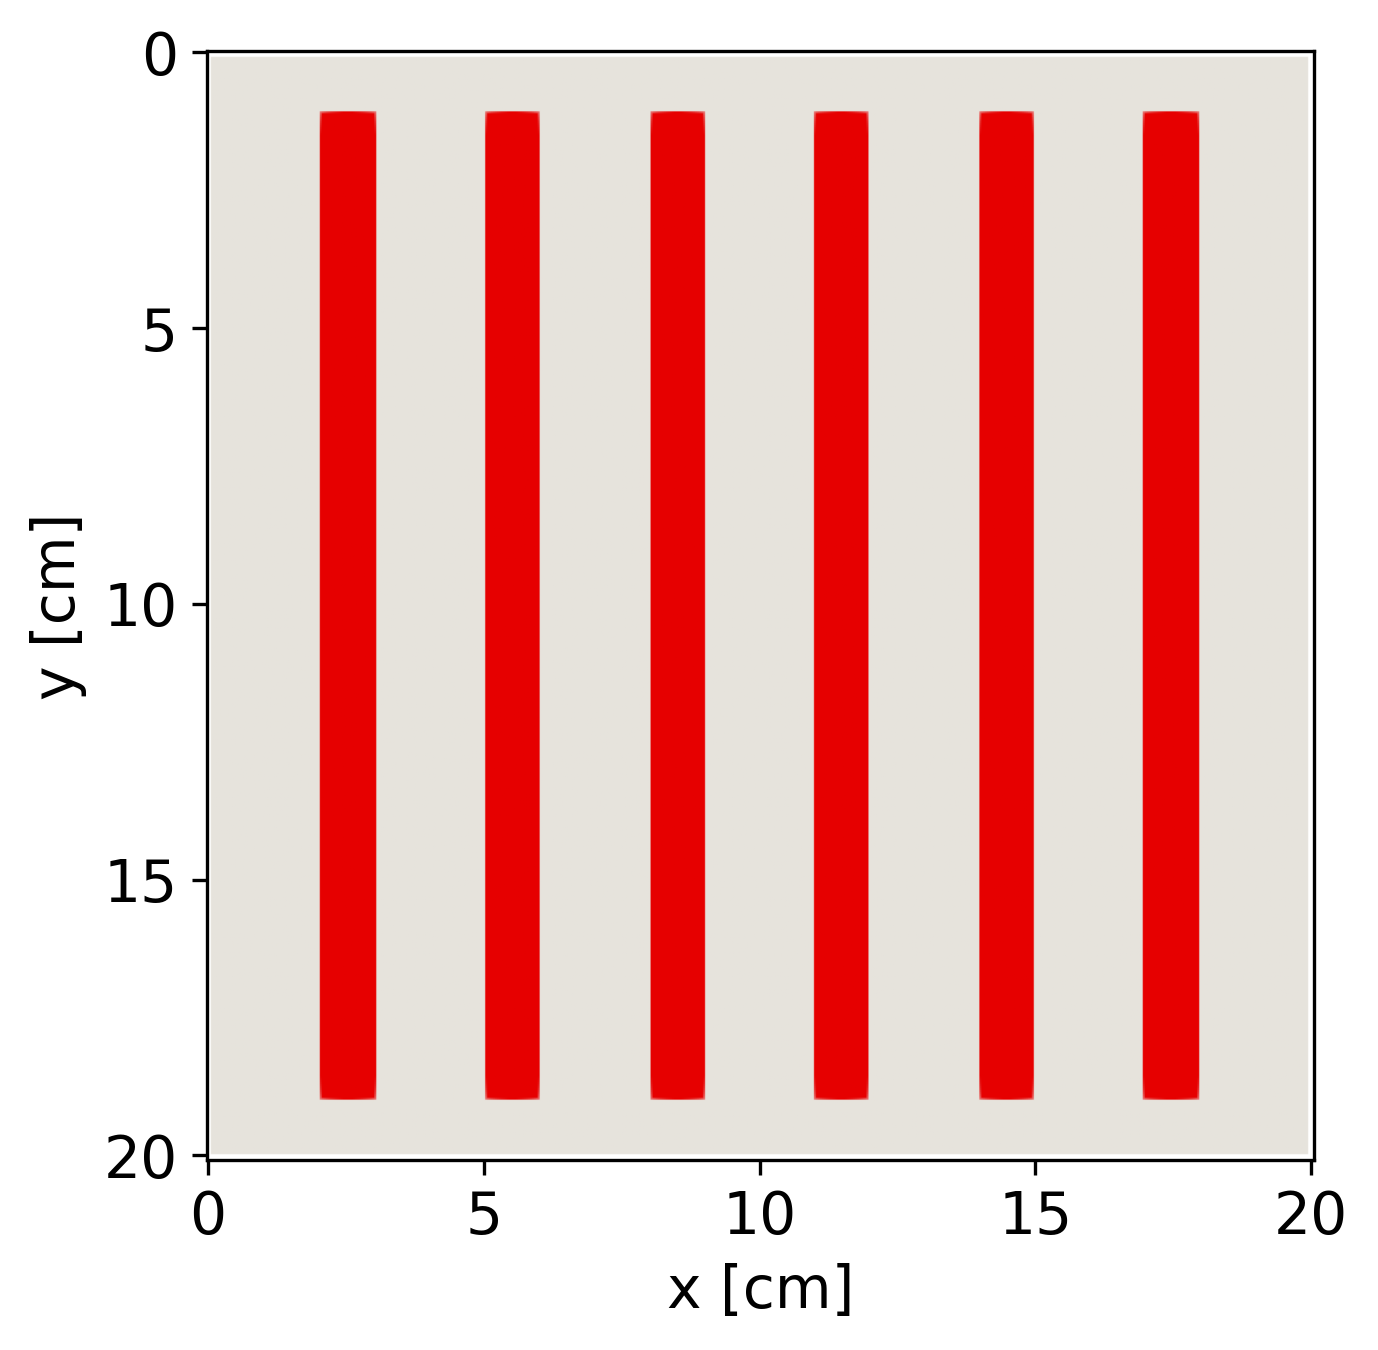
\includegraphics[width=6cm]{figures/mesh2}
        \end{center}
        \caption{Problem's geometry.}
    \end{figure}
\end{columns}
\end{frame}


\begin{frame}
\frametitle{One-group, two-dimensional eigenvalue problem (2)}

    \begin{figure}[htbp!]
        \begin{center}
            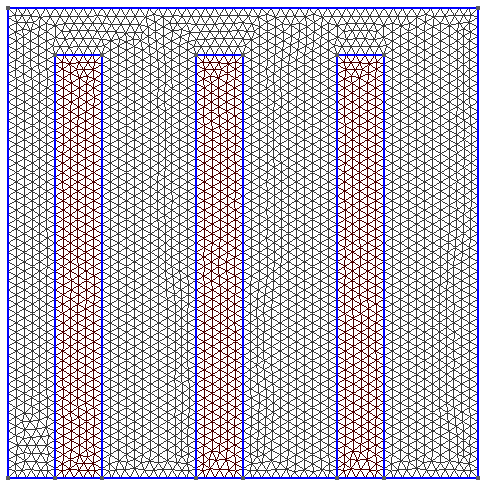
\includegraphics[width=5.5cm]{figures/mesh2b}
        \end{center}
        \caption{Gmsh 2D mesh.}
    \end{figure}
\end{frame}


\begin{frame}
\frametitle{One-group, two-dimensional eigenvalue problem (3)}

\begin{columns}
    \column[t]{5cm}
    \begin{table}[htbp!]
      \centering
      \caption{Eigenvalue comparison.}
      \begin{tabular}{lll}
      \toprule
        $k_{Ref}$ & $k_{SP_3}$  & $\Delta_{\rho}$ \\
      \midrule
        0.79862   & 0.79854     & 12        \\
      \bottomrule
      \end{tabular}
    \end{table}

    \column[t]{5cm}
    \begin{figure}[htbp!]
        \begin{center}
            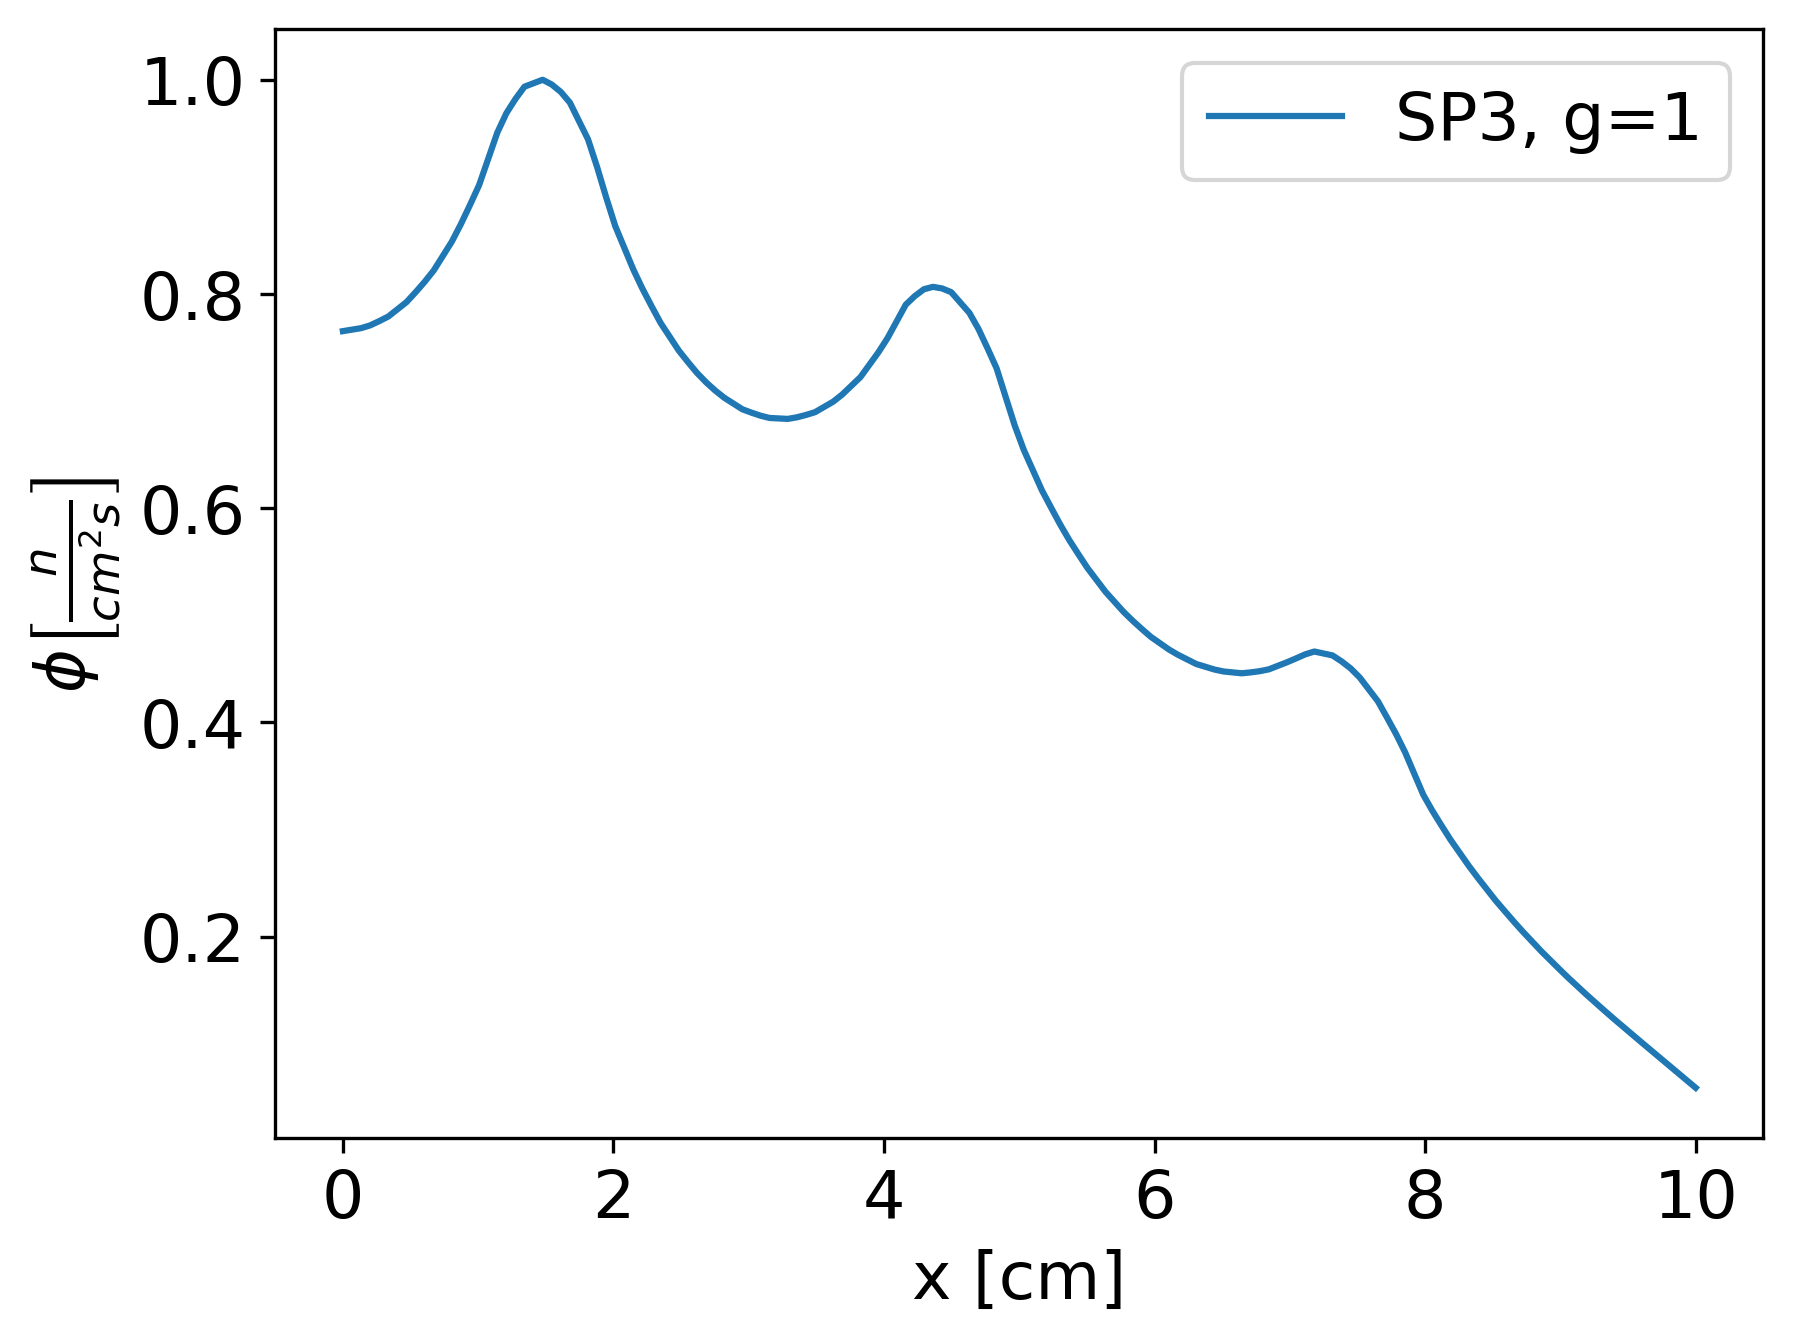
\includegraphics[width=5cm]{figures/flux-output}
        \end{center}
        \caption{Scalar flux over line at y=4.5 cm.}
    \end{figure}
\end{columns}
\end{frame}


\subsection{C5 MOX}

\begin{frame}
\frametitle{C5 MOX Benchmark}

\begin{columns}
    \column[t]{5cm}
    \begin{itemize}
        \item Exercise defined in 1994 by OECD/NEA \cite{cavarec_benchmark_1994}.
        \item Two-energy groups.
        \item Two-dimensional problem.
        \item Two types of fuel: UO$_2$, MOX.
    \end{itemize}

    \column[t]{5cm}
    \begin{figure}[htbp!]
        \begin{center}
            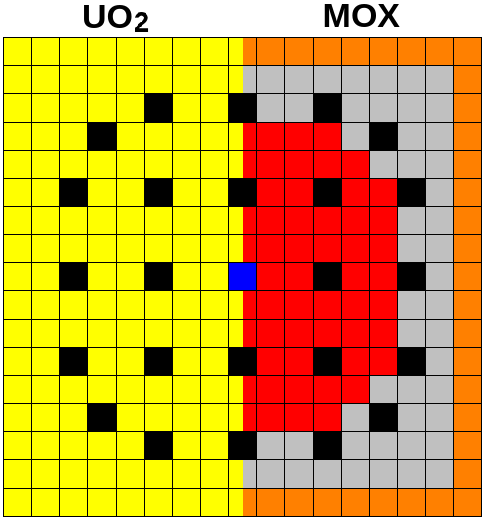
\includegraphics[width=5cm]{figures/bench-config}
        \end{center}
        \caption{2-D C5 MOX benchmark configuration. $R$ represents the reflectors. Image reproduced from \cite{capilla_applications_2009}.}
    \end{figure}
\end{columns}
\end{frame}


\begin{frame}
\frametitle{C5 MOX Benchmark (2)}

\begin{columns}
    \column[t]{5.5cm}
    \begin{figure}[htbp!]
        \begin{center}
            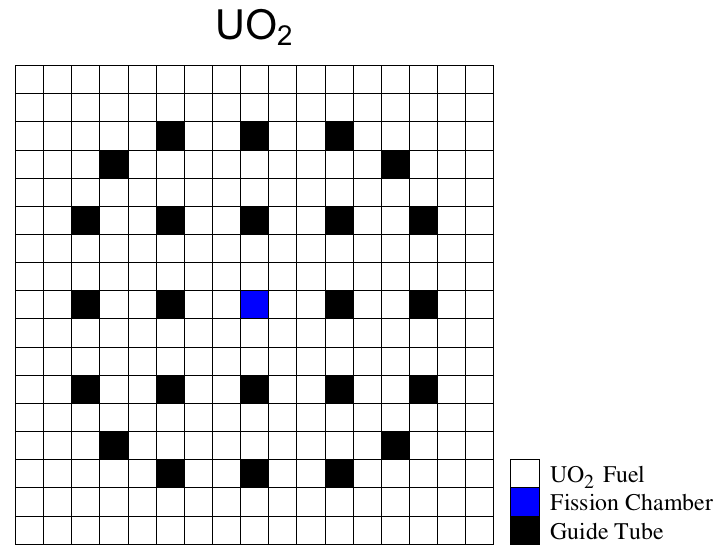
\includegraphics[width=5.5cm]{figures/bench-config2}
        \end{center}
        \caption{UO$_2$ assembly. Image reproduced from \cite{capilla_applications_2009}.}
    \end{figure}

    \column[t]{5.5cm}
    \begin{figure}[htbp!]
        \begin{center}
            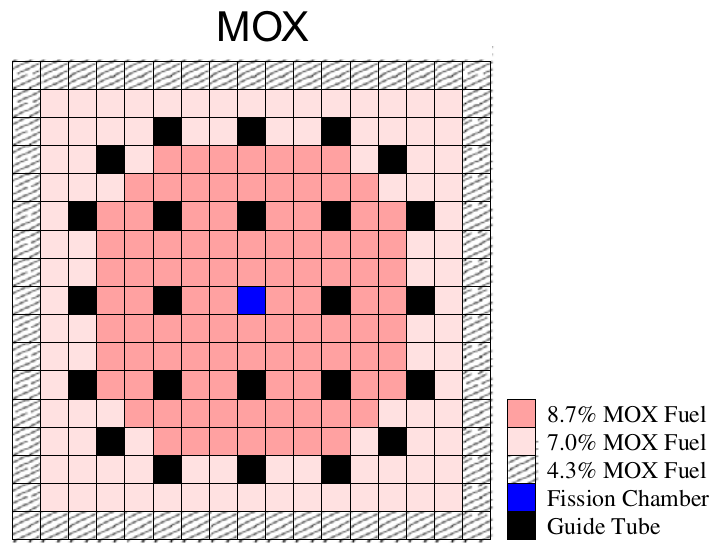
\includegraphics[width=5.5cm]{figures/bench-config3}
        \end{center}
        \caption{MOX assembly. Image reproduced from \cite{capilla_applications_2009}.}
    \end{figure}
\end{columns}
\end{frame}


\begin{frame}
\frametitle{C5 MOX Benchmark (3)}

    \begin{figure}[htbp!]
        \begin{center}
            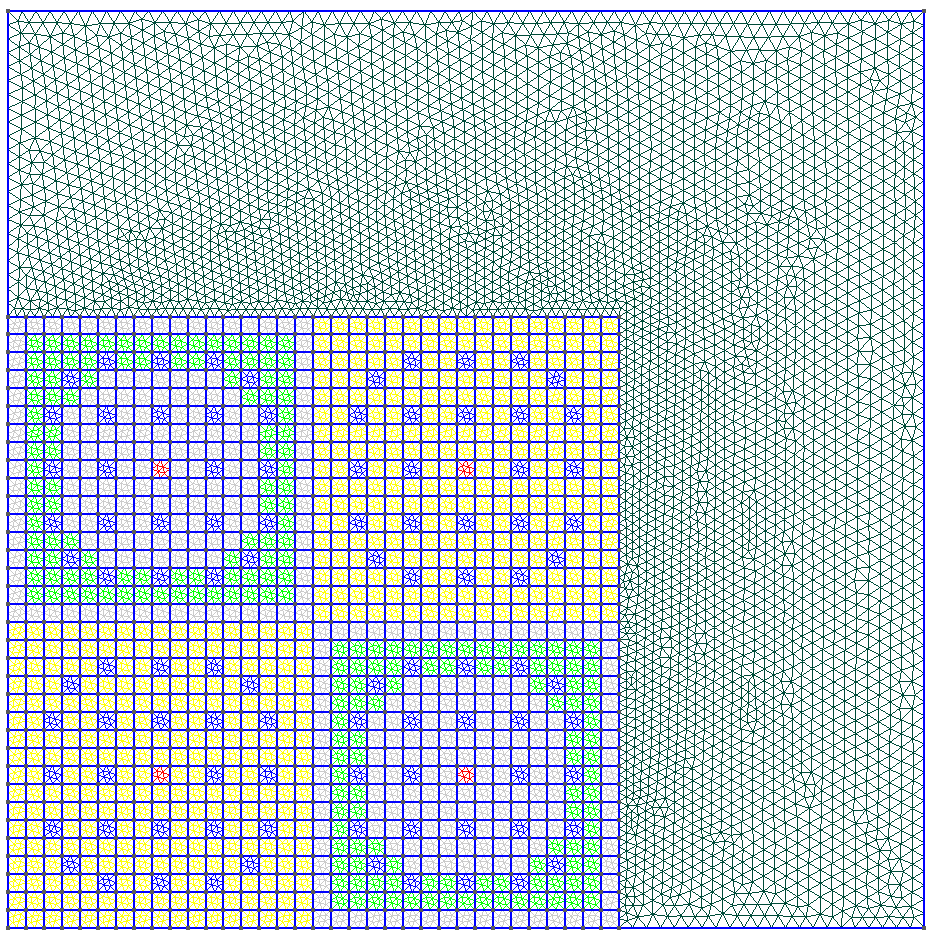
\includegraphics[width=6.cm]{figures/bench-mesh}
        \end{center}
        \caption{Gmsh 2D mesh.}
    \end{figure}

\end{frame}

% Clarification on the cross-sections

\begin{frame}
\frametitle{C5 MOX Benchmark (4)}
	\begin{table}[htbp!]
	\centering
	\begin{tabular}{lccc}
	\toprule
	 & C5G2 Benchmark      & \multicolumn{2}{c}{SP3}          \\
	\midrule
	Case & $k_{Ref}$       & $k_{SP_3}$ & $\Delta_\rho$ [pcm] \\
	\midrule
	No correction          & 0.96969  & 0.97106  & 145  \\
	Transport correction   & 0.93755  & 0.93792  &  43  \\
	\bottomrule
	\end{tabular}
	\label{tab:2d-keff}
	\end{table}
\end{frame}

% Figure with fluxes

\begin{frame}
\frametitle{C5 MOX Benchmark (5)}

    \begin{figure}[htbp!]
        \begin{center}
            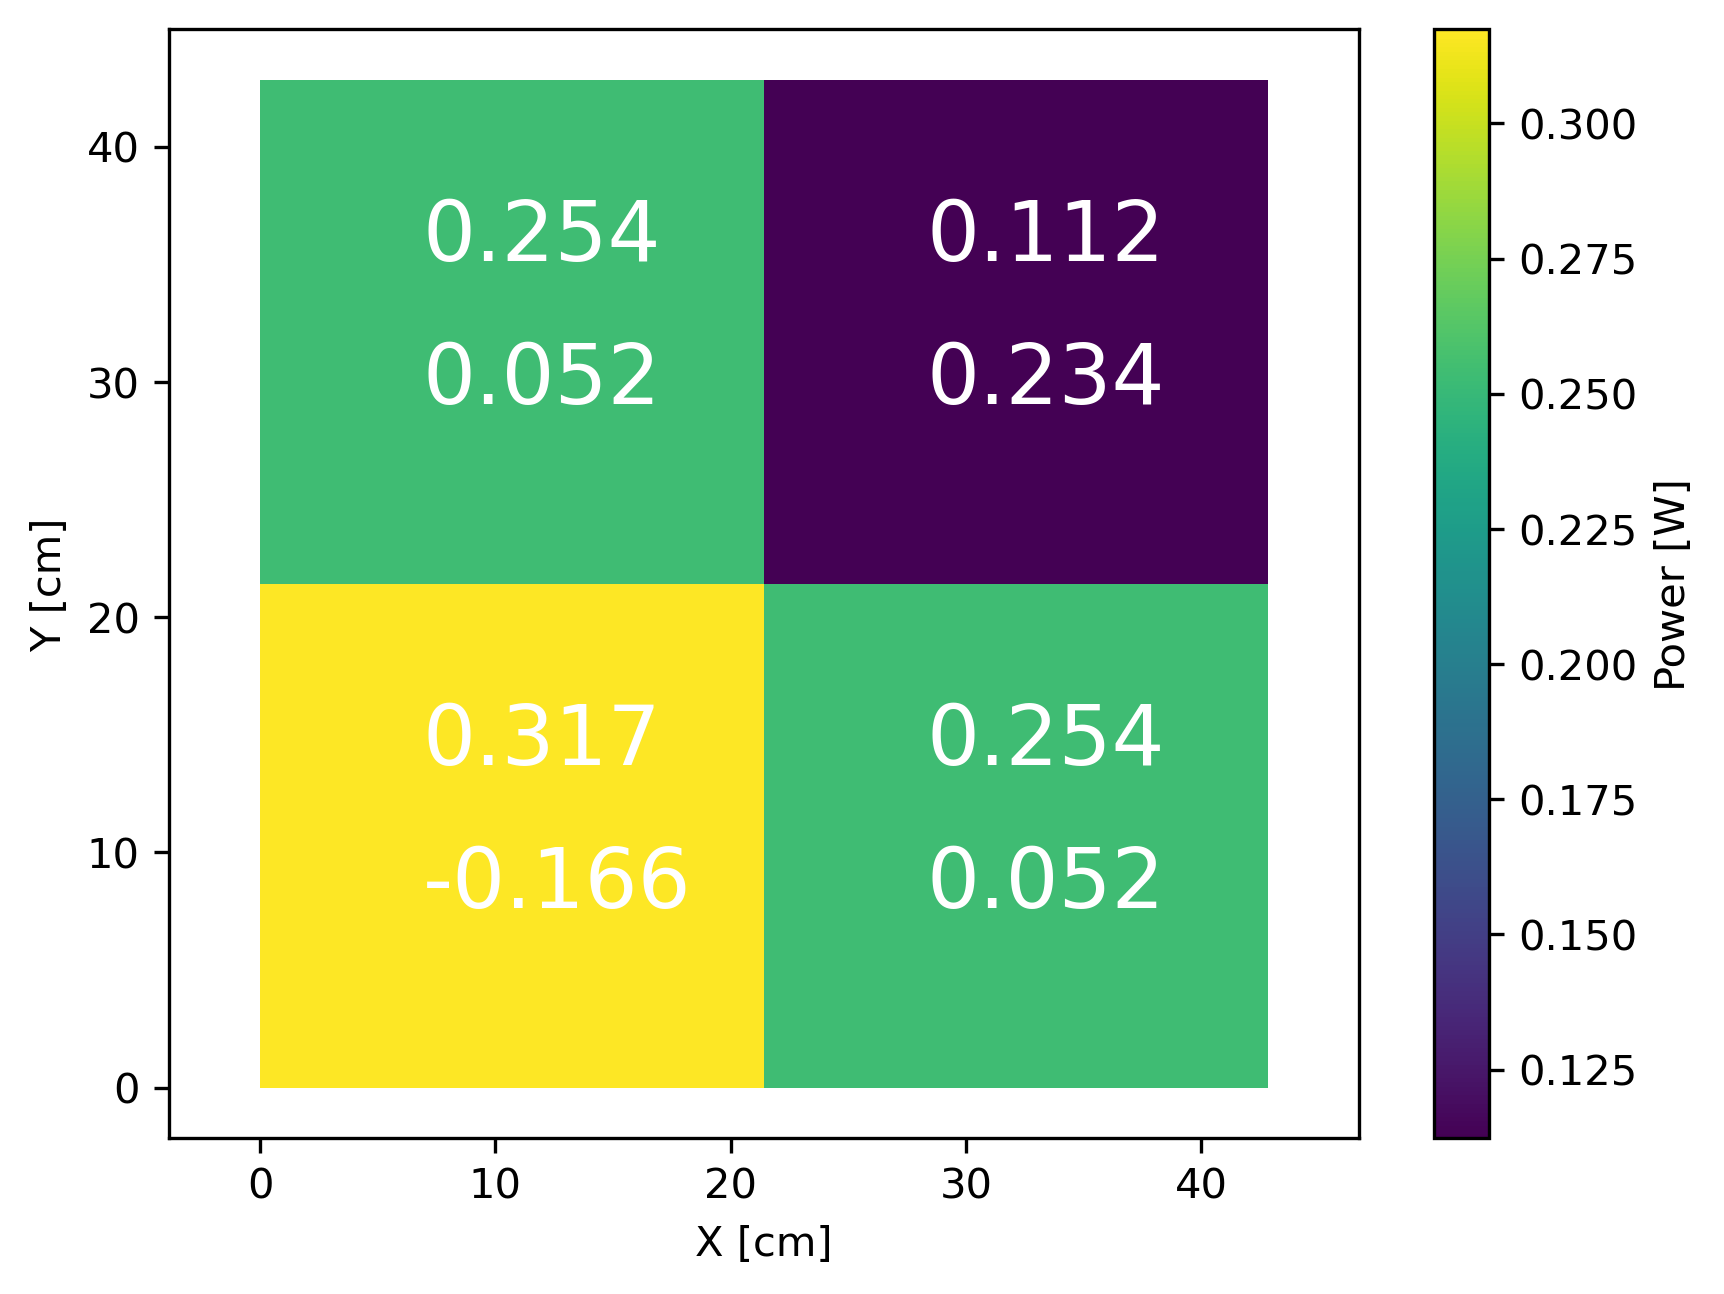
\includegraphics[width=6.cm]{figures/distrib}
        \end{center}
        \caption{Assembly power distribution. Top: assembly power. Bottom: relative difference expressed in \%.}
    \end{figure}

\end{frame}


% \section{Future studies}
% \input{future}

\section{Future work}
\subsection{Conclusions}

\begin{frame}
\frametitle{Conclusions}

    \begin{itemize}
        \item 

    \end{itemize}
\end{frame}


\subsection{Acknowledgement}

\begin{frame}
\frametitle{Acknowledgement}

This research was being performed using funding received from the DOE Office of Nuclear Energy’s University Program (Project 20-19693, DE-NE0008972) ’Evaluation of micro-reactor requirements and performance in an existing well-characterized micro-grid’.

\end{frame}


\subsection{Questions}

\begin{frame}
  \begin{center}
    \Huge{\textbf{Thank you.\\ Questions?}}
  \end{center}
\end{frame}


\begin{frame}[allowframebreaks]
  \frametitle{References}
  \bibliographystyle{plain}
  {\footnotesize \bibliography{bibliography.bib} }
\end{frame}

\end{document}
